% Commutative diagram with edges passing under/over
% Jan 7, 2009, Stefan Kottwitz
% http://texblog.net
\documentclass[landscape]{article}
\usepackage{tikz}
\usepackage[paperwidth=15cm,paperheight=7.5cm,hmargin=0.2cm,vmargin=0.5cm]{geometry}
\usetikzlibrary{matrix}
\begin{document}

\begin{tikzpicture}

\pgfmathsetmacro{\cubex}{0.1}
\pgfmathsetmacro{\cubey}{4}
\pgfmathsetmacro{\cubez}{5}

\pgfmathsetmacro{\multx}{1.5}
\pgfmathsetmacro{\divyz}{1.4}

\definecolor{convfill}{RGB}{255,255,255}
\definecolor{convline}{RGB}{0,0,0}

\definecolor{conv2fill}{RGB}{255,255,255}
\definecolor{conv2line}{RGB}{25,23,230}

\definecolor{maxline}{RGB}{255,0,0}
\definecolor{maxfill}{RGB}{255,255,255}

\definecolor{fcfill}{RGB}{255,255,255}
\definecolor{fcline}{RGB}{6,185,251}

\definecolor{softmaxfill}{RGB}{255,255,255}
\definecolor{softmaxline}{RGB}{191,115,16}

\definecolor{minmaxfill}{RGB}{255,255,255}
\definecolor{minmaxline}{RGB}{40,151,28}

\pgfmathsetmacro{\x}{0}
\pgfmathsetmacro{\offset}{0.08}

\pgfmathsetmacro{\xx}{0.5}
\pgfmathsetmacro{\vgg}{1.5}

\node[inner sep=0pt,cm={0.35 ,0.5 ,0 ,1  ,(0 cm,0 cm)}] (image) at (-1,0)
    {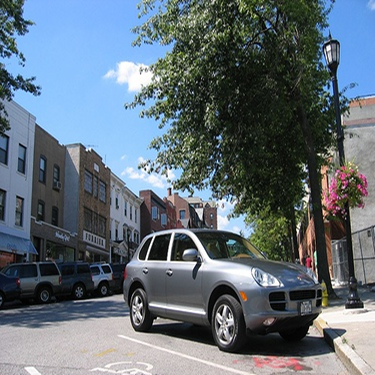
\includegraphics[width=\cubey cm]{images/003348_2}};
    
\node[text width=3cm] at (\x+\xx/2-\xx-0.6,\cubey/2+0.2,\cubez/2-\cubez) {\scriptsize $h' \!\! \times \! w' \!\! \times \! 3$};

%% conv1-1
\draw[convline,fill=convfill] (\x+\xx/2,\cubey/2,\cubez/2) -- ++(-\cubex,0,0) -- ++(0,-\cubey,0) -- ++(\cubex,0,0) -- cycle;
\draw[convline,fill=convfill] (\x+\xx/2,\cubey/2,\cubez/2) -- ++(0-\xx,0,-\cubez) -- ++(0,-\cubey,0) -- ++(0+\xx,0,\cubez) -- cycle;
\draw[convline,fill=convfill] (\x+\xx/2,\cubey/2,\cubez/2) -- ++(-\cubex,0,0) -- ++(0-\xx,0,-\cubez) -- ++(\cubex,0,0) -- cycle;

\draw[convline,fill=convfill,densely dotted] (\x+\xx/2,\cubey/2,\cubez/2) -- ++(-\cubex,0,0) -- ++(0,-\cubey/\vgg,0) -- ++(\cubex,0,0) -- cycle;
\draw[convline,fill=convfill,densely dotted] (\x+\xx/2,\cubey/2,\cubez/2) -- ++(0-\xx/\vgg,0,-\cubez/\vgg) -- ++(0,-\cubey/\vgg,0) -- ++(0+\xx/\vgg,0,\cubez/\vgg) -- cycle;
\draw[convline,fill=convfill,densely dotted] (\x+\xx/2,\cubey/2,\cubez/2) -- ++(-\cubex,0,0) -- ++(0-\xx/\vgg,0,-\cubez/\vgg) -- ++(\cubex,0,0) -- cycle;

% conv1-2
\pgfmathsetmacro{\x}{\x + \cubex + \offset}
\draw[convline,fill=convfill] (\x+\xx/2,\cubey/2,\cubez/2) -- ++(-\cubex,0,0) -- ++(0,-\cubey,0) -- ++(\cubex,0,0) -- cycle;
\draw[convline,fill=convfill] (\x+\xx/2,\cubey/2,\cubez/2) -- ++(0-\xx,0,-\cubez) -- ++(0,-\cubey,0) -- ++(0+\xx,0,\cubez) -- cycle;
\draw[convline,fill=convfill] (\x+\xx/2,\cubey/2,\cubez/2) -- ++(-\cubex,0,0) -- ++(0-\xx,0,-\cubez) -- ++(\cubex,0,0) -- cycle;

\draw[convline,fill=convfill,densely dotted] (\x+\xx/2,\cubey/2,\cubez/2) -- ++(-\cubex,0,0) -- ++(0,-\cubey/\vgg,0) -- ++(\cubex,0,0) -- cycle;
\draw[convline,fill=convfill,densely dotted] (\x+\xx/2,\cubey/2,\cubez/2) -- ++(0-\xx/\vgg,0,-\cubez/\vgg) -- ++(0,-\cubey/\vgg,0) -- ++(0+\xx/\vgg,0,\cubez/\vgg) -- cycle;
\draw[convline,fill=convfill,densely dotted] (\x+\xx/2,\cubey/2,\cubez/2) -- ++(-\cubex,0,0) -- ++(0-\xx/\vgg,0,-\cubez/\vgg) -- ++(\cubex,0,0) -- cycle;

\node[text width=3cm] at (\x+\xx/2-\xx+0.7,\cubey/2+0.2,\cubez/2-\cubez) {\scriptsize $h' \!\! \times \! w' \!\! \times \! 64$};

% pool1
\pgfmathsetmacro{\cubey}{\cubey/\divyz}
\pgfmathsetmacro{\cubez}{\cubez/\divyz}
\pgfmathsetmacro{\x}{\x + \cubex + \offset}
\pgfmathsetmacro{\xx}{\xx/\divyz}
\draw[maxline,fill=maxfill] (\x+\xx/2,\cubey/2,\cubez/2) -- ++(-\cubex,0,0) -- ++(0,-\cubey,0) -- ++(\cubex,0,0) -- cycle;
\draw[maxline,fill=maxfill] (\x+\xx/2,\cubey/2,\cubez/2) -- ++(0-\xx,0,-\cubez) -- ++(0,-\cubey,0) -- ++(0+\xx,0,\cubez) -- cycle;
\draw[maxline,fill=maxfill] (\x+\xx/2,\cubey/2,\cubez/2) -- ++(-\cubex,0,0) -- ++(0-\xx,0,-\cubez) -- ++(\cubex,0,0) -- cycle;

\draw[maxline,fill=maxfill,densely dotted] (\x+\xx/2,\cubey/2,\cubez/2) -- ++(-\cubex,0,0) -- ++(0,-\cubey/\vgg,0) -- ++(\cubex,0,0) -- cycle;
\draw[maxline,fill=maxfill,densely dotted] (\x+\xx/2,\cubey/2,\cubez/2) -- ++(0-\xx/\vgg,0,-\cubez/\vgg) -- ++(0,-\cubey/\vgg,0) -- ++(0+\xx/\vgg,0,\cubez/\vgg) -- cycle;
\draw[maxline,fill=maxfill,densely dotted] (\x+\xx/2,\cubey/2,\cubez/2) -- ++(-\cubex,0,0) -- ++(0-\xx/\vgg,0,-\cubez/\vgg) -- ++(\cubex,0,0) -- cycle;

% conv2-1
\pgfmathsetmacro{\cubex}{\cubex*\multx}
\pgfmathsetmacro{\x}{\x + \cubex + \offset}
\draw[convline,fill=convfill] (\x+\xx/2,\cubey/2,\cubez/2) -- ++(-\cubex,0,0) -- ++(0,-\cubey,0) -- ++(\cubex,0,0) -- cycle;
\draw[convline,fill=convfill] (\x+\xx/2,\cubey/2,\cubez/2) -- ++(0-\xx,0,-\cubez) -- ++(0,-\cubey,0) -- ++(0+\xx,0,\cubez) -- cycle;
\draw[convline,fill=convfill] (\x+\xx/2,\cubey/2,\cubez/2) -- ++(-\cubex,0,0) -- ++(0-\xx,0,-\cubez) -- ++(\cubex,0,0) -- cycle;

\draw[convline,fill=convfill,densely dotted] (\x+\xx/2,\cubey/2,\cubez/2) -- ++(-\cubex,0,0) -- ++(0,-\cubey/\vgg,0) -- ++(\cubex,0,0) -- cycle;
\draw[convline,fill=convfill,densely dotted] (\x+\xx/2,\cubey/2,\cubez/2) -- ++(0-\xx/\vgg,0,-\cubez/\vgg) -- ++(0,-\cubey/\vgg,0) -- ++(0+\xx/\vgg,0,\cubez/\vgg) -- cycle;
\draw[convline,fill=convfill,densely dotted] (\x+\xx/2,\cubey/2,\cubez/2) -- ++(-\cubex,0,0) -- ++(0-\xx/\vgg,0,-\cubez/\vgg) -- ++(\cubex,0,0) -- cycle;

% conv2-2
\pgfmathsetmacro{\x}{\x + \cubex + \offset}
\draw[convline,fill=convfill] (\x+\xx/2,\cubey/2,\cubez/2) -- ++(-\cubex,0,0) -- ++(0,-\cubey,0) -- ++(\cubex,0,0) -- cycle;
\draw[convline,fill=convfill] (\x+\xx/2,\cubey/2,\cubez/2) -- ++(0-\xx,0,-\cubez) -- ++(0,-\cubey,0) -- ++(0+\xx,0,\cubez) -- cycle;
\draw[convline,fill=convfill] (\x+\xx/2,\cubey/2,\cubez/2) -- ++(-\cubex,0,0) -- ++(0-\xx,0,-\cubez) -- ++(\cubex,0,0) -- cycle;

\draw[convline,fill=convfill,densely dotted] (\x+\xx/2,\cubey/2,\cubez/2) -- ++(-\cubex,0,0) -- ++(0,-\cubey/\vgg,0) -- ++(\cubex,0,0) -- cycle;
\draw[convline,fill=convfill,densely dotted] (\x+\xx/2,\cubey/2,\cubez/2) -- ++(0-\xx/\vgg,0,-\cubez/\vgg) -- ++(0,-\cubey/\vgg,0) -- ++(0+\xx/\vgg,0,\cubez/\vgg) -- cycle;
\draw[convline,fill=convfill,densely dotted] (\x+\xx/2,\cubey/2,\cubez/2) -- ++(-\cubex,0,0) -- ++(0-\xx/\vgg,0,-\cubez/\vgg) -- ++(\cubex,0,0) -- cycle;

\node at (\x+\xx/2-0.07,\cubey/2+0.22,\cubez/2-\cubez) {\scriptsize $\frac{h'}{2} \!\! \times \!\! \frac{w'}{2} \!\! \times \!\! 128$};

% pool2
\pgfmathsetmacro{\cubey}{\cubey/\divyz}
\pgfmathsetmacro{\cubez}{\cubez/\divyz}
\pgfmathsetmacro{\x}{\x + \cubex + \offset}
\pgfmathsetmacro{\xx}{\xx/\divyz}
\draw[maxline,fill=maxfill] (\x+\xx/2,\cubey/2,\cubez/2) -- ++(-\cubex,0,0) -- ++(0,-\cubey,0) -- ++(\cubex,0,0) -- cycle;
\draw[maxline,fill=maxfill] (\x+\xx/2,\cubey/2,\cubez/2) -- ++(0-\xx,0,-\cubez) -- ++(0,-\cubey,0) -- ++(0+\xx,0,\cubez) -- cycle;
\draw[maxline,fill=maxfill] (\x+\xx/2,\cubey/2,\cubez/2) -- ++(-\cubex,0,0) -- ++(0-\xx,0,-\cubez) -- ++(\cubex,0,0) -- cycle;

\draw[maxline,fill=maxfill,densely dotted] (\x+\xx/2,\cubey/2,\cubez/2) -- ++(-\cubex,0,0) -- ++(0,-\cubey/\vgg,0) -- ++(\cubex,0,0) -- cycle;
\draw[maxline,fill=maxfill,densely dotted] (\x+\xx/2,\cubey/2,\cubez/2) -- ++(0-\xx/\vgg,0,-\cubez/\vgg) -- ++(0,-\cubey/\vgg,0) -- ++(0+\xx/\vgg,0,\cubez/\vgg) -- cycle;
\draw[maxline,fill=maxfill,densely dotted] (\x+\xx/2,\cubey/2,\cubez/2) -- ++(-\cubex,0,0) -- ++(0-\xx/\vgg,0,-\cubez/\vgg) -- ++(\cubex,0,0) -- cycle;


% conv3-1
\pgfmathsetmacro{\cubex}{\cubex*\multx}
\pgfmathsetmacro{\x}{\x + \cubex + \offset}
\draw[convline,fill=convfill] (\x+\xx/2,\cubey/2,\cubez/2) -- ++(-\cubex,0,0) -- ++(0,-\cubey,0) -- ++(\cubex,0,0) -- cycle;
\draw[convline,fill=convfill] (\x+\xx/2,\cubey/2,\cubez/2) -- ++(0-\xx,0,-\cubez) -- ++(0,-\cubey,0) -- ++(0+\xx,0,\cubez) -- cycle;
\draw[convline,fill=convfill] (\x+\xx/2,\cubey/2,\cubez/2) -- ++(-\cubex,0,0) -- ++(0-\xx,0,-\cubez) -- ++(\cubex,0,0) -- cycle;

\draw[convline,fill=convfill,densely dotted] (\x+\xx/2,\cubey/2,\cubez/2) -- ++(-\cubex,0,0) -- ++(0,-\cubey/\vgg,0) -- ++(\cubex,0,0) -- cycle;
\draw[convline,fill=convfill,densely dotted] (\x+\xx/2,\cubey/2,\cubez/2) -- ++(0-\xx/\vgg,0,-\cubez/\vgg) -- ++(0,-\cubey/\vgg,0) -- ++(0+\xx/\vgg,0,\cubez/\vgg) -- cycle;
\draw[convline,fill=convfill,densely dotted] (\x+\xx/2,\cubey/2,\cubez/2) -- ++(-\cubex,0,0) -- ++(0-\xx/\vgg,0,-\cubez/\vgg) -- ++(\cubex,0,0) -- cycle;

% conv3-2
\pgfmathsetmacro{\x}{\x + \cubex + \offset}
\draw[convline,fill=convfill] (\x+\xx/2,\cubey/2,\cubez/2) -- ++(-\cubex,0,0) -- ++(0,-\cubey,0) -- ++(\cubex,0,0) -- cycle;
\draw[convline,fill=convfill] (\x+\xx/2,\cubey/2,\cubez/2) -- ++(0-\xx,0,-\cubez) -- ++(0,-\cubey,0) -- ++(0+\xx,0,\cubez) -- cycle;
\draw[convline,fill=convfill] (\x+\xx/2,\cubey/2,\cubez/2) -- ++(-\cubex,0,0) -- ++(0-\xx,0,-\cubez) -- ++(\cubex,0,0) -- cycle;

\draw[convline,fill=convfill,densely dotted] (\x+\xx/2,\cubey/2,\cubez/2) -- ++(-\cubex,0,0) -- ++(0,-\cubey/\vgg,0) -- ++(\cubex,0,0) -- cycle;
\draw[convline,fill=convfill,densely dotted] (\x+\xx/2,\cubey/2,\cubez/2) -- ++(0-\xx/\vgg,0,-\cubez/\vgg) -- ++(0,-\cubey/\vgg,0) -- ++(0+\xx/\vgg,0,\cubez/\vgg) -- cycle;
\draw[convline,fill=convfill,densely dotted] (\x+\xx/2,\cubey/2,\cubez/2) -- ++(-\cubex,0,0) -- ++(0-\xx/\vgg,0,-\cubez/\vgg) -- ++(\cubex,0,0) -- cycle;

\node at (\x+\xx/2-0.2,\cubey/2+0.22,\cubez/2-\cubez) {\scriptsize $\frac{h'}{4} \!\! \times \!\! \frac{w'}{4} \!\! \times \!\! 256$};

% conv3-3
\pgfmathsetmacro{\x}{\x + \cubex + \offset}
\draw[convline,fill=convfill] (\x+\xx/2,\cubey/2,\cubez/2) -- ++(-\cubex,0,0) -- ++(0,-\cubey,0) -- ++(\cubex,0,0) -- cycle;
\draw[convline,fill=convfill] (\x+\xx/2,\cubey/2,\cubez/2) -- ++(0-\xx,0,-\cubez) -- ++(0,-\cubey,0) -- ++(0+\xx,0,\cubez) -- cycle;
\draw[convline,fill=convfill] (\x+\xx/2,\cubey/2,\cubez/2) -- ++(-\cubex,0,0) -- ++(0-\xx,0,-\cubez) -- ++(\cubex,0,0) -- cycle;

\draw[convline,fill=convfill,densely dotted] (\x+\xx/2,\cubey/2,\cubez/2) -- ++(-\cubex,0,0) -- ++(0,-\cubey/\vgg,0) -- ++(\cubex,0,0) -- cycle;
\draw[convline,fill=convfill,densely dotted] (\x+\xx/2,\cubey/2,\cubez/2) -- ++(0-\xx/\vgg,0,-\cubez/\vgg) -- ++(0,-\cubey/\vgg,0) -- ++(0+\xx/\vgg,0,\cubez/\vgg) -- cycle;
\draw[convline,fill=convfill,densely dotted] (\x+\xx/2,\cubey/2,\cubez/2) -- ++(-\cubex,0,0) -- ++(0-\xx/\vgg,0,-\cubez/\vgg) -- ++(\cubex,0,0) -- cycle;


% pool3
\pgfmathsetmacro{\cubey}{\cubey/\divyz}
\pgfmathsetmacro{\cubez}{\cubez/\divyz}
\pgfmathsetmacro{\x}{\x + \cubex + \offset}
\pgfmathsetmacro{\xx}{\xx/\divyz}
\draw[maxline,fill=maxfill] (\x+\xx/2,\cubey/2,\cubez/2) -- ++(-\cubex,0,0) -- ++(0,-\cubey,0) -- ++(\cubex,0,0) -- cycle;
\draw[maxline,fill=maxfill] (\x+\xx/2,\cubey/2,\cubez/2) -- ++(0-\xx,0,-\cubez) -- ++(0,-\cubey,0) -- ++(0+\xx,0,\cubez) -- cycle;
\draw[maxline,fill=maxfill] (\x+\xx/2,\cubey/2,\cubez/2) -- ++(-\cubex,0,0) -- ++(0-\xx,0,-\cubez) -- ++(\cubex,0,0) -- cycle;

\draw[maxline,fill=maxfill,densely dotted] (\x+\xx/2,\cubey/2,\cubez/2) -- ++(-\cubex,0,0) -- ++(0,-\cubey/\vgg,0) -- ++(\cubex,0,0) -- cycle;
\draw[maxline,fill=maxfill,densely dotted] (\x+\xx/2,\cubey/2,\cubez/2) -- ++(0-\xx/\vgg,0,-\cubez/\vgg) -- ++(0,-\cubey/\vgg,0) -- ++(0+\xx/\vgg,0,\cubez/\vgg) -- cycle;
\draw[maxline,fill=maxfill,densely dotted] (\x+\xx/2,\cubey/2,\cubez/2) -- ++(-\cubex,0,0) -- ++(0-\xx/\vgg,0,-\cubez/\vgg) -- ++(\cubex,0,0) -- cycle;


% conv4-1
\pgfmathsetmacro{\cubex}{\cubex*\multx}
\pgfmathsetmacro{\x}{\x + \cubex + \offset}
\draw[convline,fill=convfill] (\x+\xx/2,\cubey/2,\cubez/2) -- ++(-\cubex,0,0) -- ++(0,-\cubey,0) -- ++(\cubex,0,0) -- cycle;
\draw[convline,fill=convfill] (\x+\xx/2,\cubey/2,\cubez/2) -- ++(0-\xx,0,-\cubez) -- ++(0,-\cubey,0) -- ++(0+\xx,0,\cubez) -- cycle;
\draw[convline,fill=convfill] (\x+\xx/2,\cubey/2,\cubez/2) -- ++(-\cubex,0,0) -- ++(0-\xx,0,-\cubez) -- ++(\cubex,0,0) -- cycle;

\draw[convline,fill=convfill,densely dotted] (\x+\xx/2,\cubey/2,\cubez/2) -- ++(-\cubex,0,0) -- ++(0,-\cubey/\vgg,0) -- ++(\cubex,0,0) -- cycle;
\draw[convline,fill=convfill,densely dotted] (\x+\xx/2,\cubey/2,\cubez/2) -- ++(0-\xx/\vgg,0,-\cubez/\vgg) -- ++(0,-\cubey/\vgg,0) -- ++(0+\xx/\vgg,0,\cubez/\vgg) -- cycle;
\draw[convline,fill=convfill,densely dotted] (\x+\xx/2,\cubey/2,\cubez/2) -- ++(-\cubex,0,0) -- ++(0-\xx/\vgg,0,-\cubez/\vgg) -- ++(\cubex,0,0) -- cycle;

\node at (\x+\xx/2-0.1,\cubey/2+0.22,\cubez/2-\cubez) {\scriptsize $\frac{h'}{8} \!\! \times \!\! \frac{w'}{8} \!\! \times \!\! 512$};

% conv4-2
\pgfmathsetmacro{\x}{\x + \cubex + \offset}
\draw[convline,fill=convfill] (\x+\xx/2,\cubey/2,\cubez/2) -- ++(-\cubex,0,0) -- ++(0,-\cubey,0) -- ++(\cubex,0,0) -- cycle;
\draw[convline,fill=convfill] (\x+\xx/2,\cubey/2,\cubez/2) -- ++(0-\xx,0,-\cubez) -- ++(0,-\cubey,0) -- ++(0+\xx,0,\cubez) -- cycle;
\draw[convline,fill=convfill] (\x+\xx/2,\cubey/2,\cubez/2) -- ++(-\cubex,0,0) -- ++(0-\xx,0,-\cubez) -- ++(\cubex,0,0) -- cycle;

\draw[convline,fill=convfill,densely dotted] (\x+\xx/2,\cubey/2,\cubez/2) -- ++(-\cubex,0,0) -- ++(0,-\cubey/\vgg,0) -- ++(\cubex,0,0) -- cycle;
\draw[convline,fill=convfill,densely dotted] (\x+\xx/2,\cubey/2,\cubez/2) -- ++(0-\xx/\vgg,0,-\cubez/\vgg) -- ++(0,-\cubey/\vgg,0) -- ++(0+\xx/\vgg,0,\cubez/\vgg) -- cycle;
\draw[convline,fill=convfill,densely dotted] (\x+\xx/2,\cubey/2,\cubez/2) -- ++(-\cubex,0,0) -- ++(0-\xx/\vgg,0,-\cubez/\vgg) -- ++(\cubex,0,0) -- cycle;

% conv4-3
\pgfmathsetmacro{\x}{\x + \cubex + \offset}
\draw[convline,fill=convfill] (\x+\xx/2,\cubey/2,\cubez/2) -- ++(-\cubex,0,0) -- ++(0,-\cubey,0) -- ++(\cubex,0,0) -- cycle;
\draw[convline,fill=convfill] (\x+\xx/2,\cubey/2,\cubez/2) -- ++(0-\xx,0,-\cubez) -- ++(0,-\cubey,0) -- ++(0+\xx,0,\cubez) -- cycle;
\draw[convline,fill=convfill] (\x+\xx/2,\cubey/2,\cubez/2) -- ++(-\cubex,0,0) -- ++(0-\xx,0,-\cubez) -- ++(\cubex,0,0) -- cycle;

\draw[convline,fill=convfill,densely dotted] (\x+\xx/2,\cubey/2,\cubez/2) -- ++(-\cubex,0,0) -- ++(0,-\cubey/\vgg,0) -- ++(\cubex,0,0) -- cycle;
\draw[convline,fill=convfill,densely dotted] (\x+\xx/2,\cubey/2,\cubez/2) -- ++(0-\xx/\vgg,0,-\cubez/\vgg) -- ++(0,-\cubey/\vgg,0) -- ++(0+\xx/\vgg,0,\cubez/\vgg) -- cycle;
\draw[convline,fill=convfill,densely dotted] (\x+\xx/2,\cubey/2,\cubez/2) -- ++(-\cubex,0,0) -- ++(0-\xx/\vgg,0,-\cubez/\vgg) -- ++(\cubex,0,0) -- cycle;



% pool4
\pgfmathsetmacro{\cubey}{\cubey/\divyz}
\pgfmathsetmacro{\cubez}{\cubez/\divyz}
\pgfmathsetmacro{\x}{\x + \cubex + \offset}
\pgfmathsetmacro{\xx}{\xx/\divyz}
\draw[maxline,fill=maxfill] (\x+\xx/2,\cubey/2,\cubez/2) -- ++(-\cubex,0,0) -- ++(0,-\cubey,0) -- ++(\cubex,0,0) -- cycle;
\draw[maxline,fill=maxfill] (\x+\xx/2,\cubey/2,\cubez/2) -- ++(0-\xx,0,-\cubez) -- ++(0,-\cubey,0) -- ++(0+\xx,0,\cubez) -- cycle;
\draw[maxline,fill=maxfill] (\x+\xx/2,\cubey/2,\cubez/2) -- ++(-\cubex,0,0) -- ++(0-\xx,0,-\cubez) -- ++(\cubex,0,0) -- cycle;

\draw[maxline,fill=maxfill,densely dotted] (\x+\xx/2,\cubey/2,\cubez/2) -- ++(-\cubex,0,0) -- ++(0,-\cubey/\vgg,0) -- ++(\cubex,0,0) -- cycle;
\draw[maxline,fill=maxfill,densely dotted] (\x+\xx/2,\cubey/2,\cubez/2) -- ++(0-\xx/\vgg,0,-\cubez/\vgg) -- ++(0,-\cubey/\vgg,0) -- ++(0+\xx/\vgg,0,\cubez/\vgg) -- cycle;
\draw[maxline,fill=maxfill,densely dotted] (\x+\xx/2,\cubey/2,\cubez/2) -- ++(-\cubex,0,0) -- ++(0-\xx/\vgg,0,-\cubez/\vgg) -- ++(\cubex,0,0) -- cycle;

% conv5-1
\pgfmathsetmacro{\x}{\x + \cubex + \offset}
\draw[convline,fill=convfill] (\x+\xx/2,\cubey/2,\cubez/2) -- ++(-\cubex,0,0) -- ++(0,-\cubey,0) -- ++(\cubex,0,0) -- cycle;
\draw[convline,fill=convfill] (\x+\xx/2,\cubey/2,\cubez/2) -- ++(0-\xx,0,-\cubez) -- ++(0,-\cubey,0) -- ++(0+\xx,0,\cubez) -- cycle;
\draw[convline,fill=convfill] (\x+\xx/2,\cubey/2,\cubez/2) -- ++(-\cubex,0,0) -- ++(0-\xx,0,-\cubez) -- ++(\cubex,0,0) -- cycle;

\draw[convline,fill=convfill,densely dotted] (\x+\xx/2,\cubey/2,\cubez/2) -- ++(-\cubex,0,0) -- ++(0,-\cubey/\vgg,0) -- ++(\cubex,0,0) -- cycle;
\draw[convline,fill=convfill,densely dotted] (\x+\xx/2,\cubey/2,\cubez/2) -- ++(0-\xx/\vgg,0,-\cubez/\vgg) -- ++(0,-\cubey/\vgg,0) -- ++(0+\xx/\vgg,0,\cubez/\vgg) -- cycle;
\draw[convline,fill=convfill,densely dotted] (\x+\xx/2,\cubey/2,\cubez/2) -- ++(-\cubex,0,0) -- ++(0-\xx/\vgg,0,-\cubez/\vgg) -- ++(\cubex,0,0) -- cycle;

\node at (\x+\xx/2-0.1,\cubey/2+0.22,\cubez/2-\cubez) {\scriptsize $\frac{h'}{16} \!\! \times \!\! \frac{w'}{16} \!\! \times \!\! 512$};

% conv5-2
\pgfmathsetmacro{\x}{\x + \cubex + \offset}
\draw[convline,fill=convfill] (\x+\xx/2,\cubey/2,\cubez/2) -- ++(-\cubex,0,0) -- ++(0,-\cubey,0) -- ++(\cubex,0,0) -- cycle;
\draw[convline,fill=convfill] (\x+\xx/2,\cubey/2,\cubez/2) -- ++(0-\xx,0,-\cubez) -- ++(0,-\cubey,0) -- ++(0+\xx,0,\cubez) -- cycle;
\draw[convline,fill=convfill] (\x+\xx/2,\cubey/2,\cubez/2) -- ++(-\cubex,0,0) -- ++(0-\xx,0,-\cubez) -- ++(\cubex,0,0) -- cycle;

\draw[convline,fill=convfill,densely dotted] (\x+\xx/2,\cubey/2,\cubez/2) -- ++(-\cubex,0,0) -- ++(0,-\cubey/\vgg,0) -- ++(\cubex,0,0) -- cycle;
\draw[convline,fill=convfill,densely dotted] (\x+\xx/2,\cubey/2,\cubez/2) -- ++(0-\xx/\vgg,0,-\cubez/\vgg) -- ++(0,-\cubey/\vgg,0) -- ++(0+\xx/\vgg,0,\cubez/\vgg) -- cycle;
\draw[convline,fill=convfill,densely dotted] (\x+\xx/2,\cubey/2,\cubez/2) -- ++(-\cubex,0,0) -- ++(0-\xx/\vgg,0,-\cubez/\vgg) -- ++(\cubex,0,0) -- cycle;

% conv5-3
\pgfmathsetmacro{\x}{\x + \cubex + \offset}
\draw[convline,fill=convfill] (\x+\xx/2,\cubey/2,\cubez/2) -- ++(-\cubex,0,0) -- ++(0,-\cubey,0) -- ++(\cubex,0,0) -- cycle;
\draw[convline,fill=convfill] (\x+\xx/2,\cubey/2,\cubez/2) -- ++(0-\xx,0,-\cubez) -- ++(0,-\cubey,0) -- ++(0+\xx,0,\cubez) -- cycle;
\draw[convline,fill=convfill] (\x+\xx/2,\cubey/2,\cubez/2) -- ++(-\cubex,0,0) -- ++(0-\xx,0,-\cubez) -- ++(\cubex,0,0) -- cycle;

\draw[convline,fill=convfill,densely dotted] (\x+\xx/2,\cubey/2,\cubez/2) -- ++(-\cubex,0,0) -- ++(0,-\cubey/\vgg,0) -- ++(\cubex,0,0) -- cycle;
\draw[convline,fill=convfill,densely dotted] (\x+\xx/2,\cubey/2,\cubez/2) -- ++(0-\xx/\vgg,0,-\cubez/\vgg) -- ++(0,-\cubey/\vgg,0) -- ++(0+\xx/\vgg,0,\cubez/\vgg) -- cycle;
\draw[convline,fill=convfill,densely dotted] (\x+\xx/2,\cubey/2,\cubez/2) -- ++(-\cubex,0,0) -- ++(0-\xx/\vgg,0,-\cubez/\vgg) -- ++(\cubex,0,0) -- cycle;


% pool5
\pgfmathsetmacro{\cubey}{\cubey/\divyz}
\pgfmathsetmacro{\cubez}{\cubez/\divyz}
\pgfmathsetmacro{\x}{\x + \cubex + \offset}
\pgfmathsetmacro{\xx}{\xx/\divyz}
\draw[maxline,fill=maxfill] (\x+\xx/2,\cubey/2,\cubez/2) -- ++(-\cubex,0,0) -- ++(0,-\cubey,0) -- ++(\cubex,0,0) -- cycle;
\draw[maxline,fill=maxfill] (\x+\xx/2,\cubey/2,\cubez/2) -- ++(0-\xx,0,-\cubez) -- ++(0,-\cubey,0) -- ++(0+\xx,0,\cubez) -- cycle;
\draw[maxline,fill=maxfill] (\x+\xx/2,\cubey/2,\cubez/2) -- ++(-\cubex,0,0) -- ++(0-\xx,0,-\cubez) -- ++(\cubex,0,0) -- cycle;

\draw[maxline,fill=maxfill,densely dotted] (\x+\xx/2,\cubey/2,\cubez/2) -- ++(-\cubex,0,0) -- ++(0,-\cubey/\vgg,0) -- ++(\cubex,0,0) -- cycle;
\draw[maxline,fill=maxfill,densely dotted] (\x+\xx/2,\cubey/2,\cubez/2) -- ++(0-\xx/\vgg,0,-\cubez/\vgg) -- ++(0,-\cubey/\vgg,0) -- ++(0+\xx/\vgg,0,\cubez/\vgg) -- cycle;
\draw[maxline,fill=maxfill,densely dotted] (\x+\xx/2,\cubey/2,\cubez/2) -- ++(-\cubex,0,0) -- ++(0-\xx/\vgg,0,-\cubez/\vgg) -- ++(\cubex,0,0) -- cycle;

\node (sizepool5) at (\x+\xx/2-0.5,\cubey/2+1,0) {\scriptsize $\frac{h'}{32} \!\! \times \!\! \frac{w'}{32} \!\! \times \!\! 512$};

\draw[-stealth] (\x+\xx/2 -\cubex/2,\cubey/2+0.8,0)--(\x+\xx/2 -\cubex/2,\cubey/2 ,0);

% conv6
\pgfmathsetmacro{\cubex}{\cubex*2.5}
\pgfmathsetmacro{\cubey}{\cubey/\divyz}
\pgfmathsetmacro{\cubez}{\cubez/\divyz}
\pgfmathsetmacro{\x}{\x + \cubex + \offset}
\pgfmathsetmacro{\xx}{\xx/\divyz}
\draw[convline,fill=convfill] (\x+\xx/2,\cubey/2,\cubez/2) -- ++(-\cubex,0,0) -- ++(0,-\cubey,0) -- ++(\cubex,0,0) -- cycle;
\draw[convline,fill=convfill] (\x+\xx/2,\cubey/2,\cubez/2) -- ++(0-\xx,0,-\cubez) -- ++(0,-\cubey,0) -- ++(0+\xx,0,\cubez) -- cycle;
\draw[convline,fill=convfill] (\x+\xx/2,\cubey/2,\cubez/2) -- ++(-\cubex,0,0) -- ++(0-\xx,0,-\cubez) -- ++(\cubex,0,0) -- cycle;

\pgfmathsetmacro{\vgg}{\vgg*3}
\draw[convline,fill=convfill,densely dotted] (\x+\xx/2,\cubey/2,\cubez/2) -- ++(-\cubex,0,0) -- ++(0,-\cubey/\vgg,0) -- ++(\cubex,0,0) -- cycle;
\draw[convline,fill=convfill,densely dotted] (\x+\xx/2,\cubey/2,\cubez/2) -- ++(0-\xx/\vgg,0,-\cubez/\vgg) -- ++(0,-\cubey/\vgg,0) -- ++(0+\xx/\vgg,0,\cubez/\vgg) -- cycle;
\draw[convline,fill=convfill,densely dotted] (\x+\xx/2,\cubey/2,\cubez/2) -- ++(-\cubex,0,0) -- ++(0-\xx/\vgg,0,-\cubez/\vgg) -- ++(\cubex,0,0) -- cycle;

\node at (\x+\xx/2-0.7,\cubey/2+1.5,0) {\scriptsize $h \! \times \! w \! \times \! 4096$};

\draw[-stealth] (\x+\xx/2-\xx -\cubex/2,\cubey/2+1.3,0)--(\x+\xx/2-\xx -\cubex/2,\cubey/2 ,0);

% conv7
\pgfmathsetmacro{\cubex}{\cubex/2.5}
\pgfmathsetmacro{\x}{\x + \cubex + \offset}
\draw[conv2line,fill=conv2fill] (\x+\xx/2,\cubey/2,\cubez/2) -- ++(-\cubex,0,0) -- ++(0,-\cubey,0) -- ++(\cubex,0,0) -- cycle;
\draw[conv2line,fill=conv2fill] (\x+\xx/2,\cubey/2,\cubez/2) -- ++(0-\xx,0,-\cubez) -- ++(0,-\cubey,0) -- ++(0+\xx,0,\cubez) -- cycle;
\draw[conv2line,fill=conv2fill] (\x+\xx/2,\cubey/2,\cubez/2) -- ++(-\cubex,0,0) -- ++(0-\xx,0,-\cubez) -- ++(\cubex,0,0) -- cycle;

\node at (\x+\xx/2-0.2,\cubey/2+1.85,0) {\scriptsize $h \! \times \! w \! \times \! C$};
\draw[-stealth] (\x+\xx/2-\xx-0.1,\cubey/2+1.7)--(\x+\xx/2-\xx-0.1,\cubey/2 ,0);

\node at (\x+\xx/2-\xx,\cubey/2+2.7) {\scriptsize $h \!=\! \frac{h'}{32}  \!-\! 6 \qquad w \!=\! \frac{w'}{32}  \!-\! 6$};

\pgfmathsetmacro{\ya}{-1.8}
\pgfmathsetmacro{\cubexa}{\cubex*3}
\pgfmathsetmacro{\cubeya}{\cubey*2}
\pgfmathsetmacro{\cubeza}{\cubez*2}

\node[inner sep=0pt,cm={0.43 ,0.5 ,0 ,1  ,(0 cm,0 cm)}] (image) at (\x-\cubexa,\ya)
    {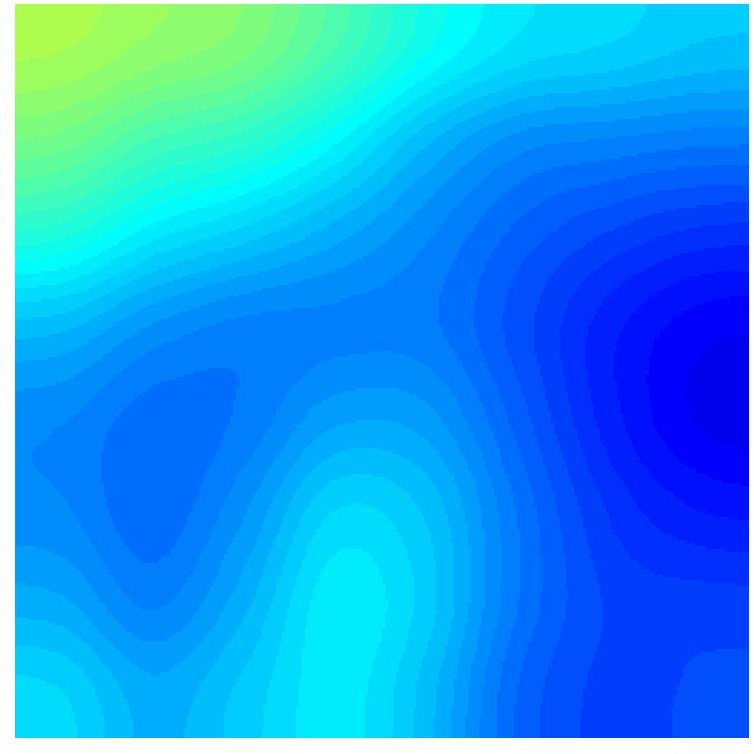
\includegraphics[width=11mm, height=11mm]{images/heatmap_boat}};
\node[inner sep=0pt,cm={0.43 ,0.5 ,0 ,1  ,(0 cm,0 cm)}] (image) at (\x-\cubexa/2,\ya)
    {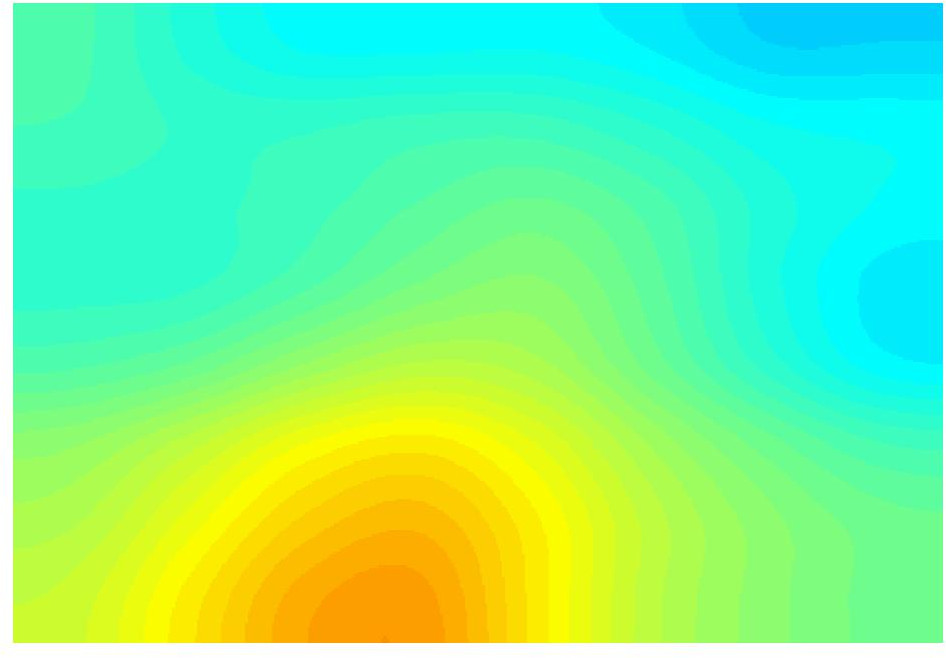
\includegraphics[width=11 mm, height=11mm]{images/heatmap_2}};
\node[inner sep=0pt,cm={0.43 ,0.5 ,0 ,1  ,(0 cm,0 cm)}] (image) at (\x,\ya)
    {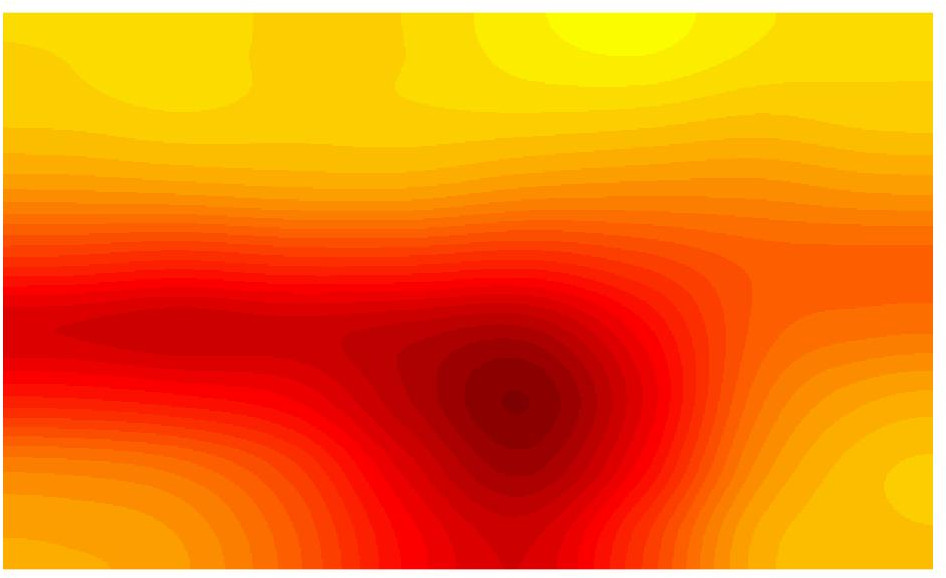
\includegraphics[width=11 mm, height=11mm]{images/heatmap_car}};
    
\draw[conv2line,fill=conv2fill,fill opacity=0] (\x+\xx/2,\ya+\cubeya/2,\cubeza/2) -- ++(-\cubexa,0,0) -- ++(0,-\cubeya,0) -- ++(\cubexa,0,0) -- cycle;
\draw[conv2line,fill=conv2fill,fill opacity=0] (\x+\xx/2,\ya+\cubeya/2,\cubeza/2) -- ++(0-\xx,0,-\cubeza) -- ++(0,-\cubeya,0) -- ++(0+\xx,0,\cubeza) -- cycle;
\draw[conv2line,fill=conv2fill,fill opacity=0] (\x+\xx/2,\ya+\cubeya/2,\cubeza/2) -- ++(-\cubexa,0,0) -- ++(0-\xx,0,-\cubeza) -- ++(\cubexa,0,0) -- cycle;


\draw[line width=0.2mm, conv2line, densely dotted] (\x+\xx/2-\cubex,-\cubey/2,\cubez/2) -- (\x+\xx/2-\cubexa-\xx,\ya+\cubeya/2,\cubeza/2-\cubeza);
\draw[line width=0.2mm, conv2line, densely dotted] (\x+\xx/2,-\cubey/2,\cubez/2) -- (\x+\xx/2-\xx,\ya+\cubeya/2,\cubeza/2-\cubeza);

\node at (\x+\xx/2-1,-2.7) {\scriptsize boat};
\node at (\x+\xx/2,-2.7) {\scriptsize car};

% minmax
\pgfmathsetmacro{\cubeyo}{\cubey}
\pgfmathsetmacro{\cubezo}{\cubez}
\pgfmathsetmacro{\cubexo}{\cubex}
\pgfmathsetmacro{\cubey}{\cubey/4}
\pgfmathsetmacro{\cubez}{\cubez/4}
\pgfmathsetmacro{\cubex}{\cubex}
\pgfmathsetmacro{\xx}{\xx/4}
\pgfmathsetmacro{\x}{\x + \cubex + 2.5 * \offset}
\draw[minmaxline,fill=minmaxfill] (\x+\xx/2,\cubey/2,\cubez/2) -- ++(-\cubex,0,0) -- ++(0,-\cubey,0) -- ++(\cubex,0,0) -- cycle;
\draw[minmaxline,fill=minmaxfill] (\x+\xx/2,\cubey/2,\cubez/2) -- ++(0-\xx,0,-\cubez) -- ++(0,-\cubey,0) -- ++(0+\xx,0,\cubez) -- cycle;
\draw[minmaxline,fill=minmaxfill] (\x+\xx/2,\cubey/2,\cubez/2) -- ++(-\cubex,0,0) -- ++(0-\xx,0,-\cubez) -- ++(\cubex,0,0) -- cycle;

\node at (\x+\xx/2-0,\cubey/2+0.22,0) {\scriptsize $1 \!\! \times \!\! 1 \!\! \times \!\! C$};

\node at (\x+\xx/2 + 2.5,0) {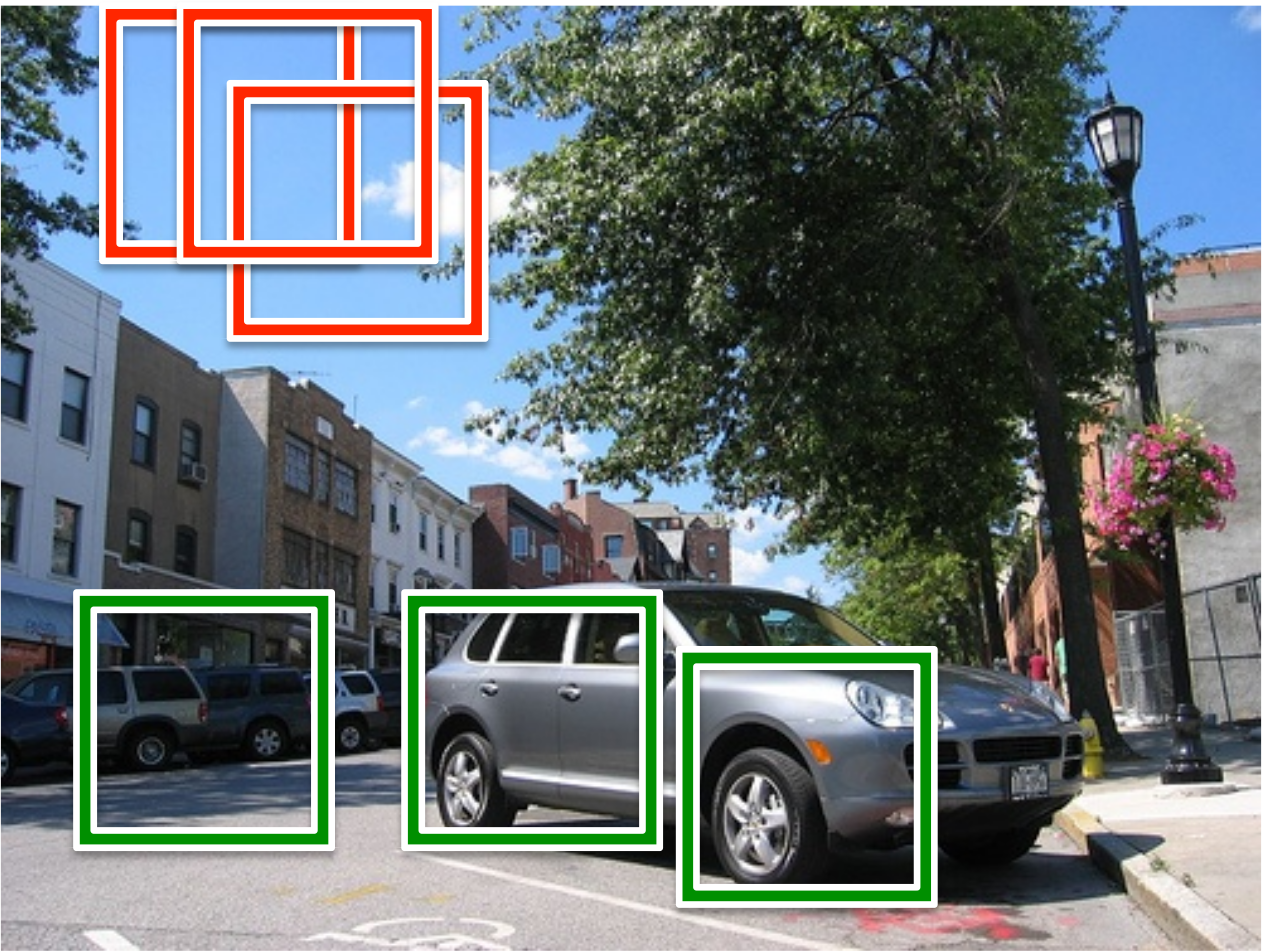
\includegraphics[height=3 cm]{images/prediction}};


\pgfmathsetmacro{\x}{\x/3.5}
\pgfmathsetmacro{\y}{-1.8}
\pgfmathsetmacro{\divyz}{\divyz*3}
\pgfmathsetmacro{\cubex}{\cubexo/8*\divyz}
\pgfmathsetmacro{\cubey}{\cubeyo/\divyz}
\pgfmathsetmacro{\cubez}{\cubezo/\divyz}
\pgfmathsetmacro{\xx}{\xx/\divyz}

\draw[convline,fill=convfill] (\x+\xx/2,\y+\cubey/2,\cubez/2) -- ++(-\cubex,0,0) -- ++(0,-\cubey,0) -- ++(\cubex,0,0) -- cycle;
\draw[convline,fill=convfill] (\x+\xx/2,\y+\cubey/2,\cubez/2) -- ++(0-\xx,0,-\cubez) -- ++(0,-\cubey,0) -- ++(0+\xx,0,\cubez) -- cycle;
\draw[convline,fill=convfill] (\x+\xx/2,\y+\cubey/2,\cubez/2) -- ++(-\cubex,0,0) -- ++(0-\xx,0,-\cubez) -- ++(\cubex,0,0) -- cycle;

\node[text width=3cm] at (\x+1.7,\y+0.05,0) {\scriptsize convolution+ReLU};

\pgfmathsetmacro{\y}{\y-0.35}
\draw[maxline,fill=maxfill] (\x+\xx/2,\y+\cubey/2,\cubez/2) -- ++(-\cubex,0,0) -- ++(0,-\cubey,0) -- ++(\cubex,0,0) -- cycle;
\draw[maxline,fill=maxfill] (\x+\xx/2,\y+\cubey/2,\cubez/2) -- ++(0-\xx,0,-\cubez) -- ++(0,-\cubey,0) -- ++(0+\xx,0,\cubez) -- cycle;
\draw[maxline,fill=maxfill] (\x+\xx/2,\y+\cubey/2,\cubez/2) -- ++(-\cubex,0,0) -- ++(0-\xx,0,-\cubez) -- ++(\cubex,0,0) -- cycle;

\node[text width=3cm] at (\x+1.7,\y+0.05,0) {\scriptsize max pooling};

\pgfmathsetmacro{\y}{\y-0.35}
\draw[conv2line,fill=conv2fill] (\x+\xx/2,\y+\cubey/2,\cubez/2) -- ++(-\cubex,0,0) -- ++(0,-\cubey,0) -- ++(\cubex,0,0) -- cycle;
\draw[conv2line,fill=conv2fill] (\x+\xx/2,\y+\cubey/2,\cubez/2) -- ++(0-\xx,0,-\cubez) -- ++(0,-\cubey,0) -- ++(0+\xx,0,\cubez) -- cycle;
\draw[conv2line,fill=conv2fill] (\x+\xx/2,\y+\cubey/2,\cubez/2) -- ++(-\cubex,0,0) -- ++(0-\xx,0,-\cubez) -- ++(\cubex,0,0) -- cycle;

\node[text width=3cm] at (\x+1.7,\y+0.05,0) {\scriptsize convolution};

\pgfmathsetmacro{\y}{\y-0.35}
\draw[minmaxline,fill=minmaxfill] (\x+\xx/2,\y+\cubey/2,\cubez/2) -- ++(-\cubex,0,0) -- ++(0,-\cubey,0) -- ++(\cubex,0,0) -- cycle;
\draw[minmaxline,fill=minmaxfill] (\x+\xx/2,\y+\cubey/2,\cubez/2) -- ++(0-\xx,0,-\cubez) -- ++(0,-\cubey,0) -- ++(0+\xx,0,\cubez) -- cycle;
\draw[minmaxline,fill=minmaxfill] (\x+\xx/2,\y+\cubey/2,\cubez/2) -- ++(-\cubex,0,0) -- ++(0-\xx,0,-\cubez) -- ++(\cubex,0,0) -- cycle;

\node[text width=4cm] at (\x+2.2,\y,0) {\scriptsize WELDON pooling };

\end{tikzpicture}

\end{document}